\subsubsection{Relais}\label{sec:relai}
\begin{figwindow}[1,r,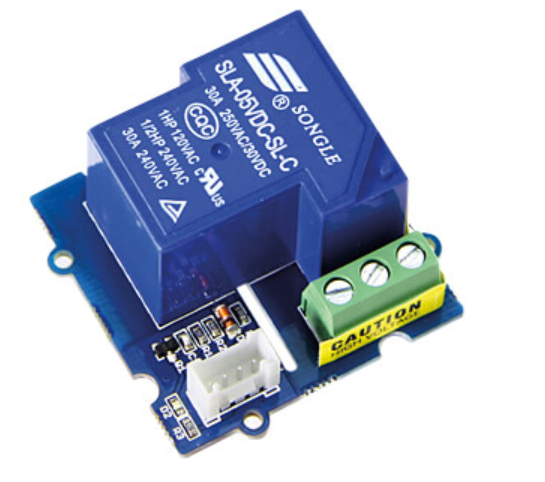
\includegraphics[scale=0.5]{image/relai.jpg.png},{Relais\autocite{Relais}}]
Mit einem Relais kann man mit kleinen Spannungen große Spannungen schalten. Ein Relais\autocite{Relais} besteht aus einer Spule und einem beweglichen Kontakt. Wenn Strom durch die Spule fließt, erzeugt sie ein Magnetfeld, das den Kontakt beeinflusst. Dadurch ändert sich der Zustand des Schaltkontakts, und ein elektrischer Pfad wird geöffnet oder geschlossen. Relais dienen dazu, mit einem schwachen Steuersignal einen starken elektrischen Stromkreis zu steuern oder zu schalten. Relais werden in unserer DA verwendet, um mit dem Raspberry Netzspannungen zu schalten. 
Für unsere Anwendung brauchen wir das GRV RELAY SPDT30, dieses ist ein hochwertiges einpoliges Zweiwege-Relais mit hoher\\ Schaltleistung. Es ist für Betriebsspannungen von 4,75 bis 5,25 V und Schaltströme von bis zu 30 A bei 250 V AC oder 30 V DC ausgelegt. Das Relais ist kompatibel mit den Schnittstellen vom Raspberry Pi, verfügt über eine schnelle Einschaltzeit von maximal 15ms und eine Betriebstemperatur von -25 bis +75°C.  Eingesetzt wird es in der Teststation für die Steuerung des Netzteils und für die UV Lampe.
\end{figwindow}